\chapter{Ideen}

\renewcommand{\figurename}{Abb.}

\section{Skizzen}

    \begin{figure}[H]
        \centering
        \begin{minipage}[H]{7cm}
        \centering
        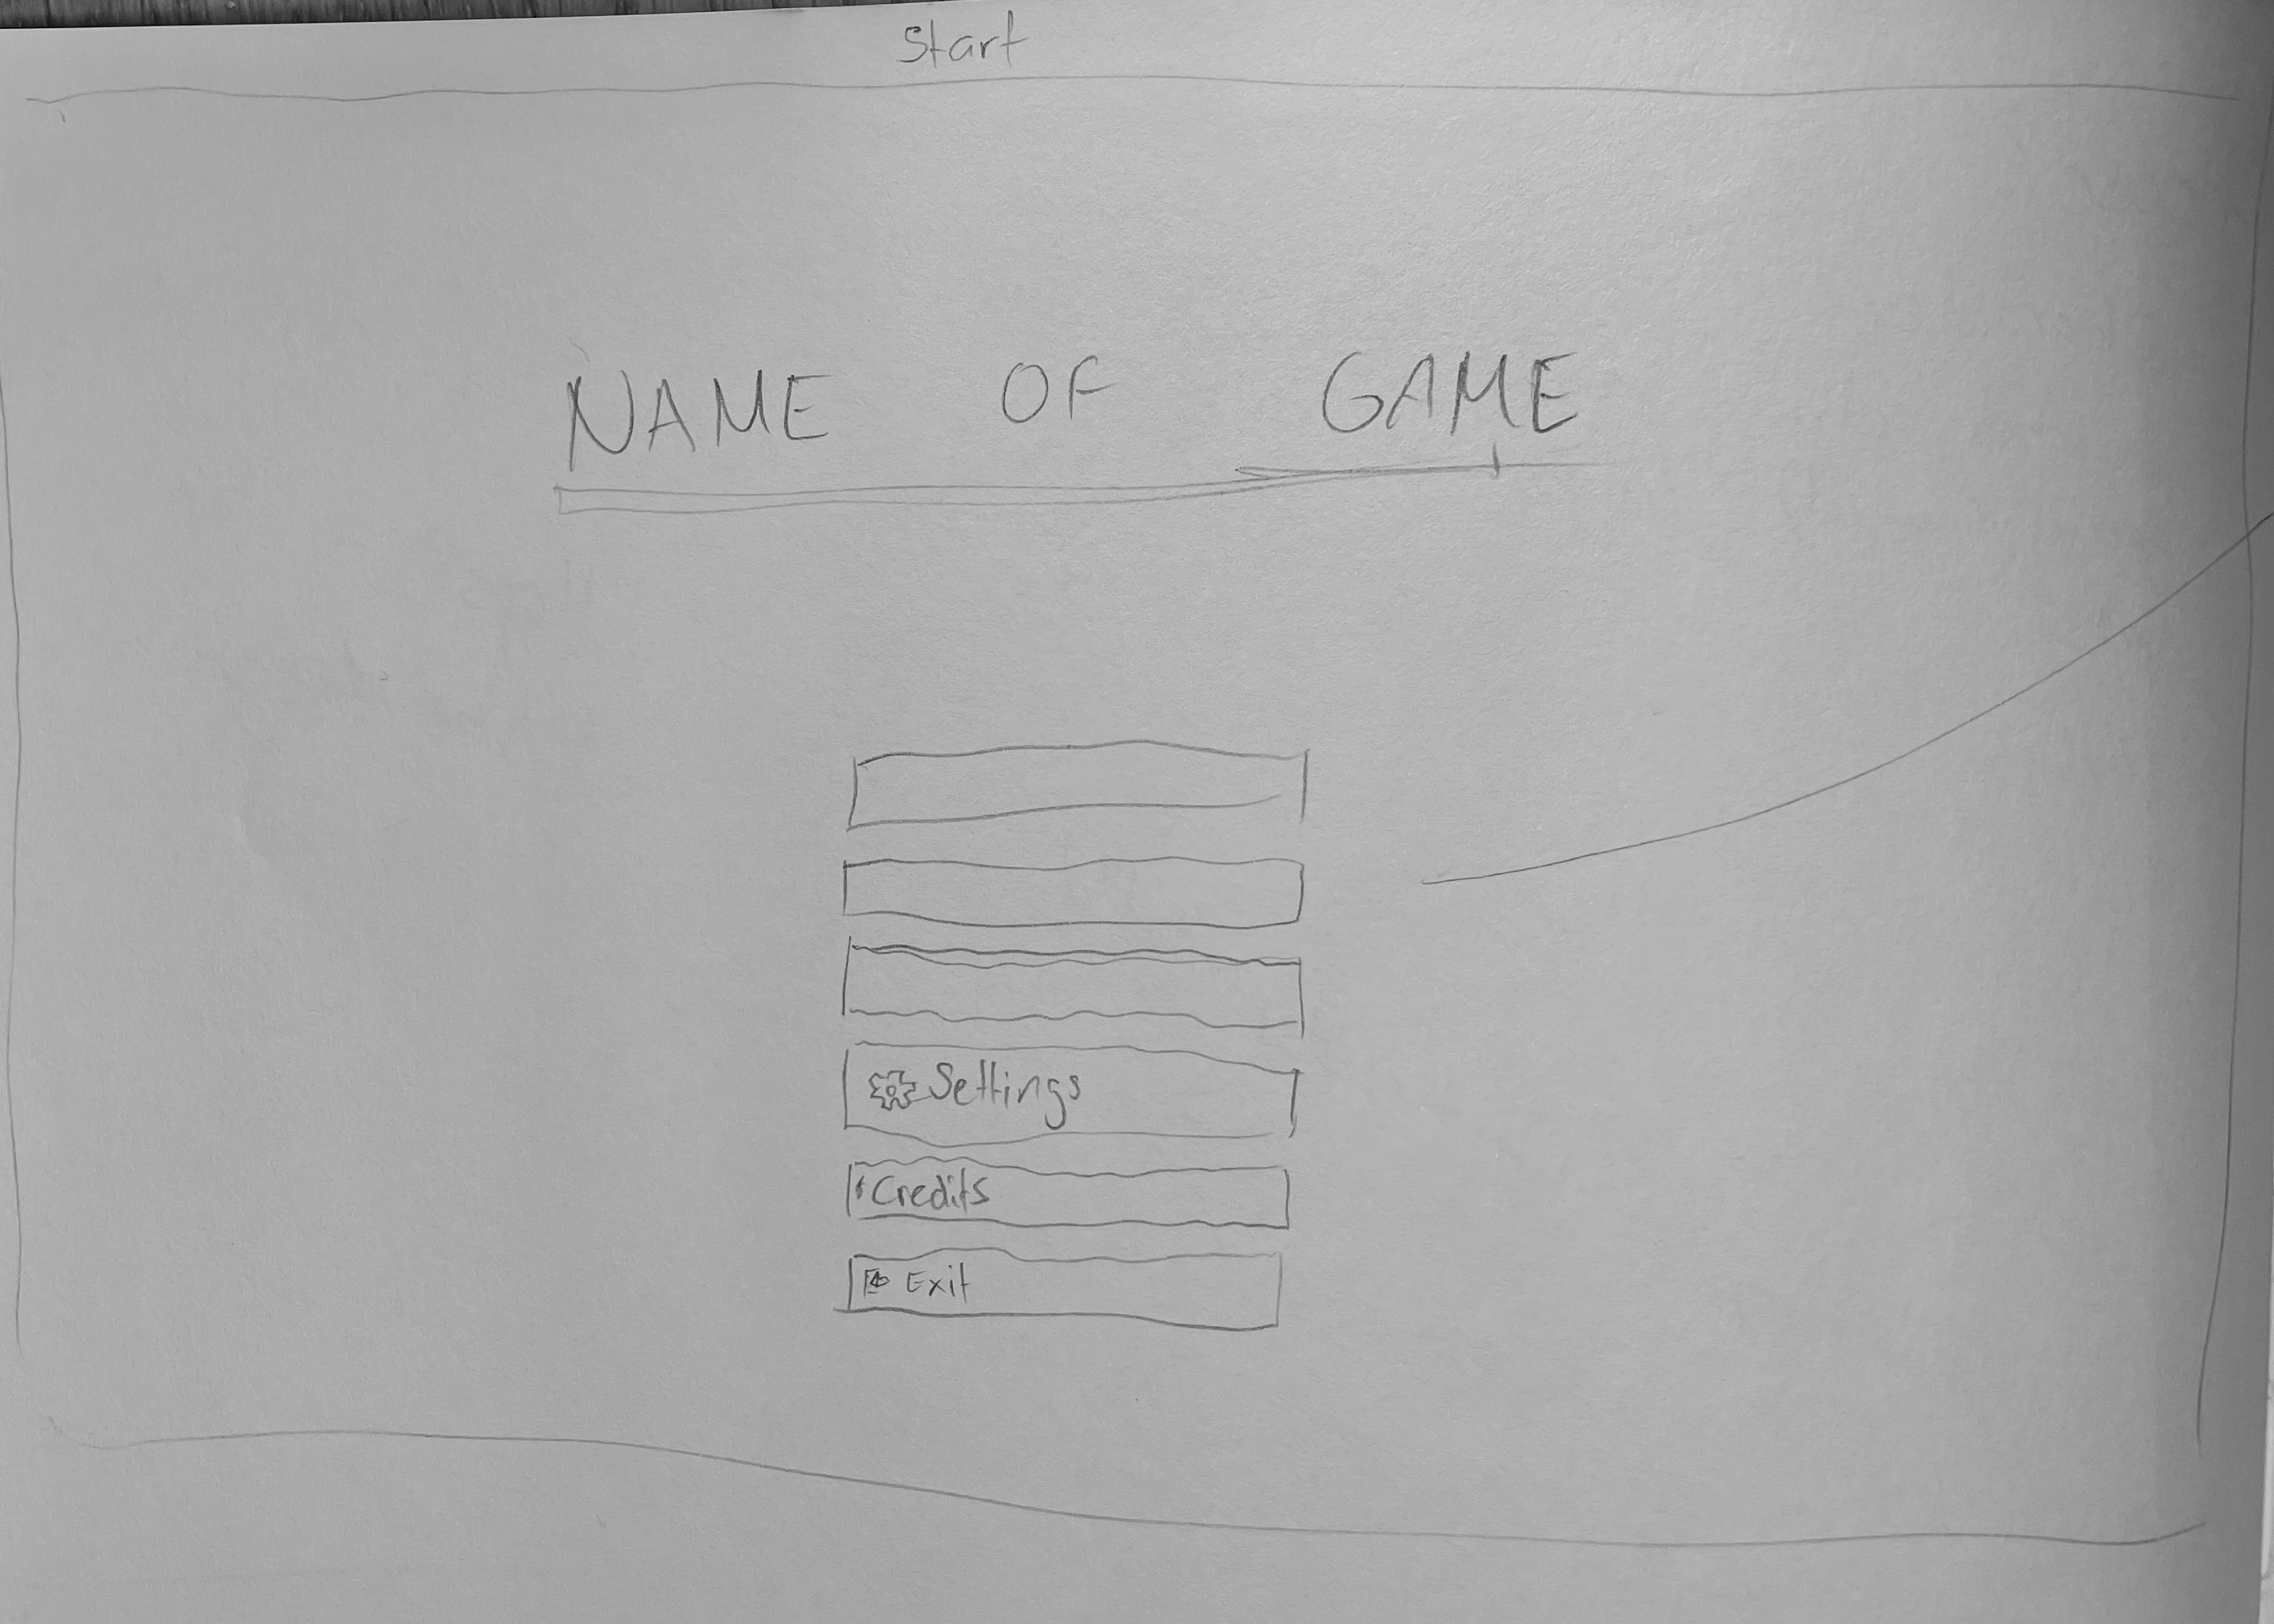
\includegraphics[width=7cm]{resources/Sk_startpage.jpeg}\\
        \caption{Aufbau der Startseite}
        \end{minipage}\hfill
        \begin{minipage}[H]{7cm}
        \centering
        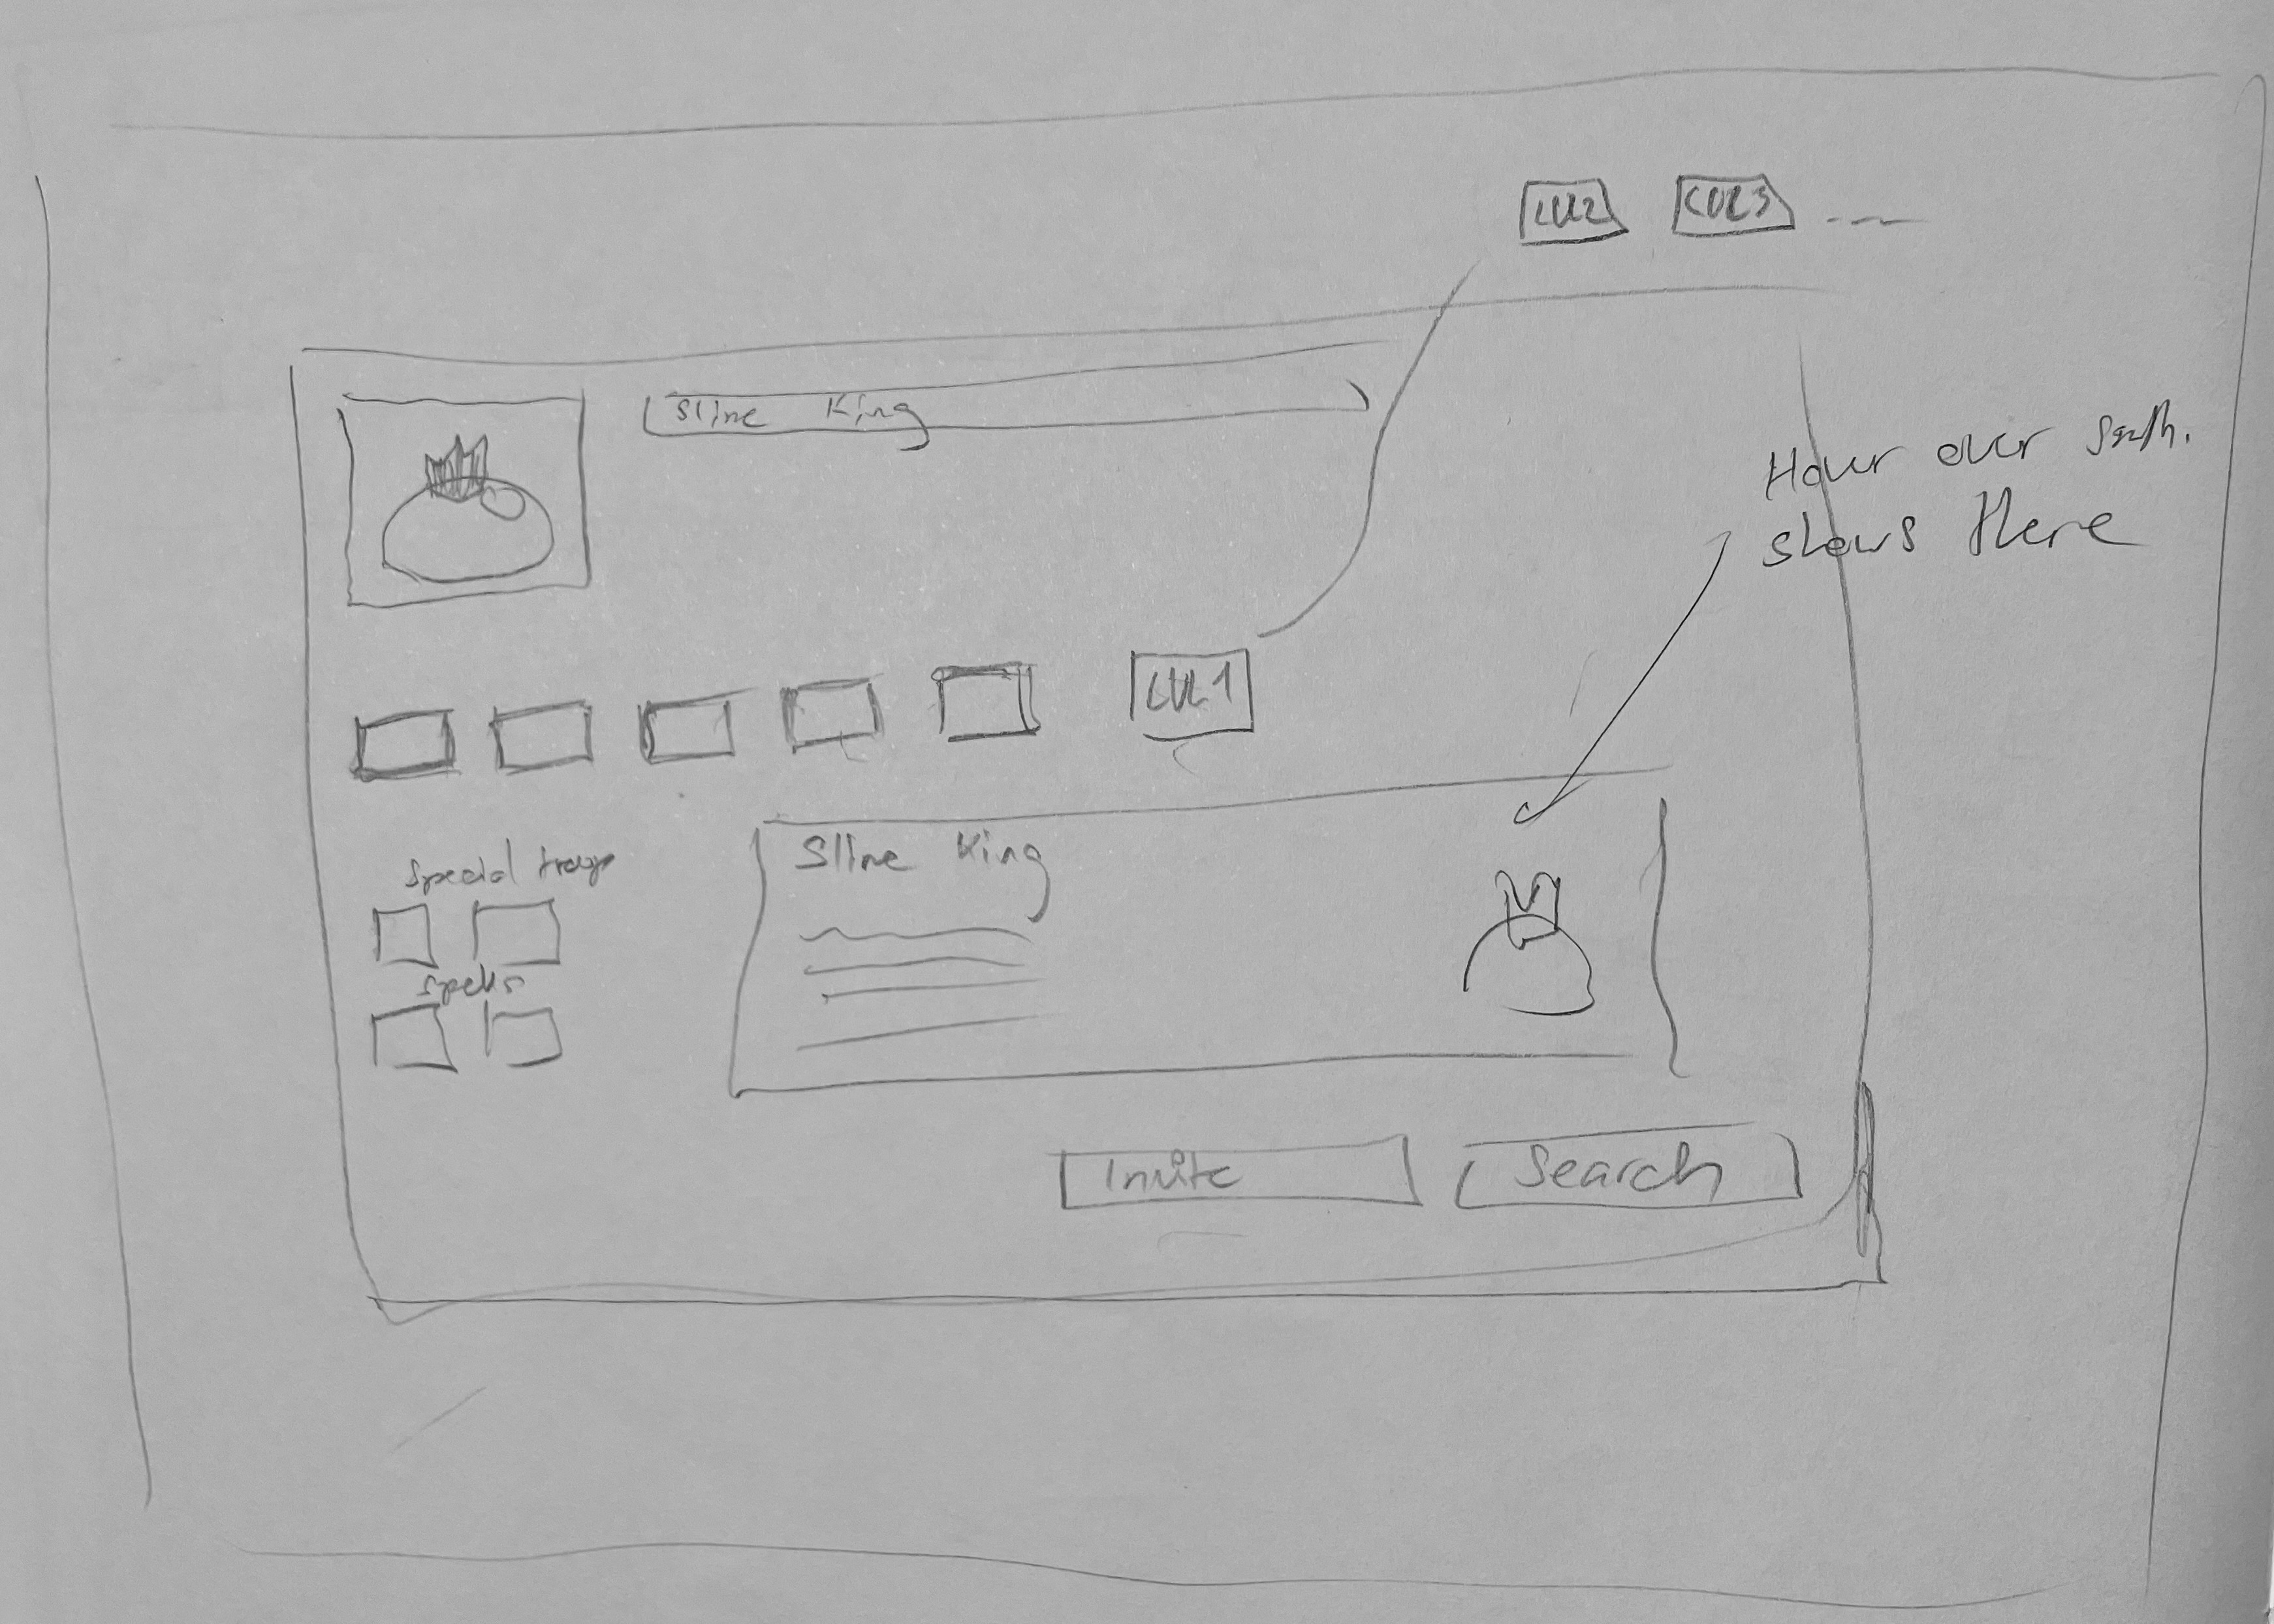
\includegraphics[width=7cm]{resources/SK_auswahl.jpeg}\\
        \caption{Aufbau bei der Deckerstellung}
        \end{minipage}
    \end{figure}
    %\begin{figure}
    %    \centering
    %    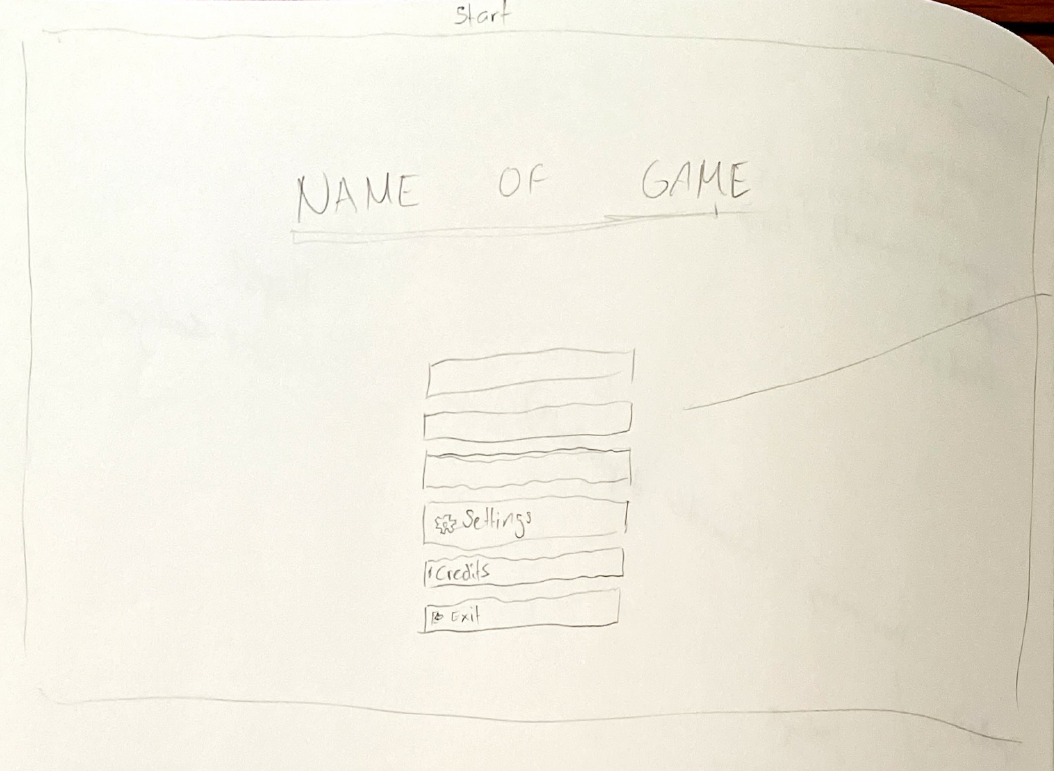
\includegraphics[width=7cm]{resources/SK_startpage.jpeg} \quad 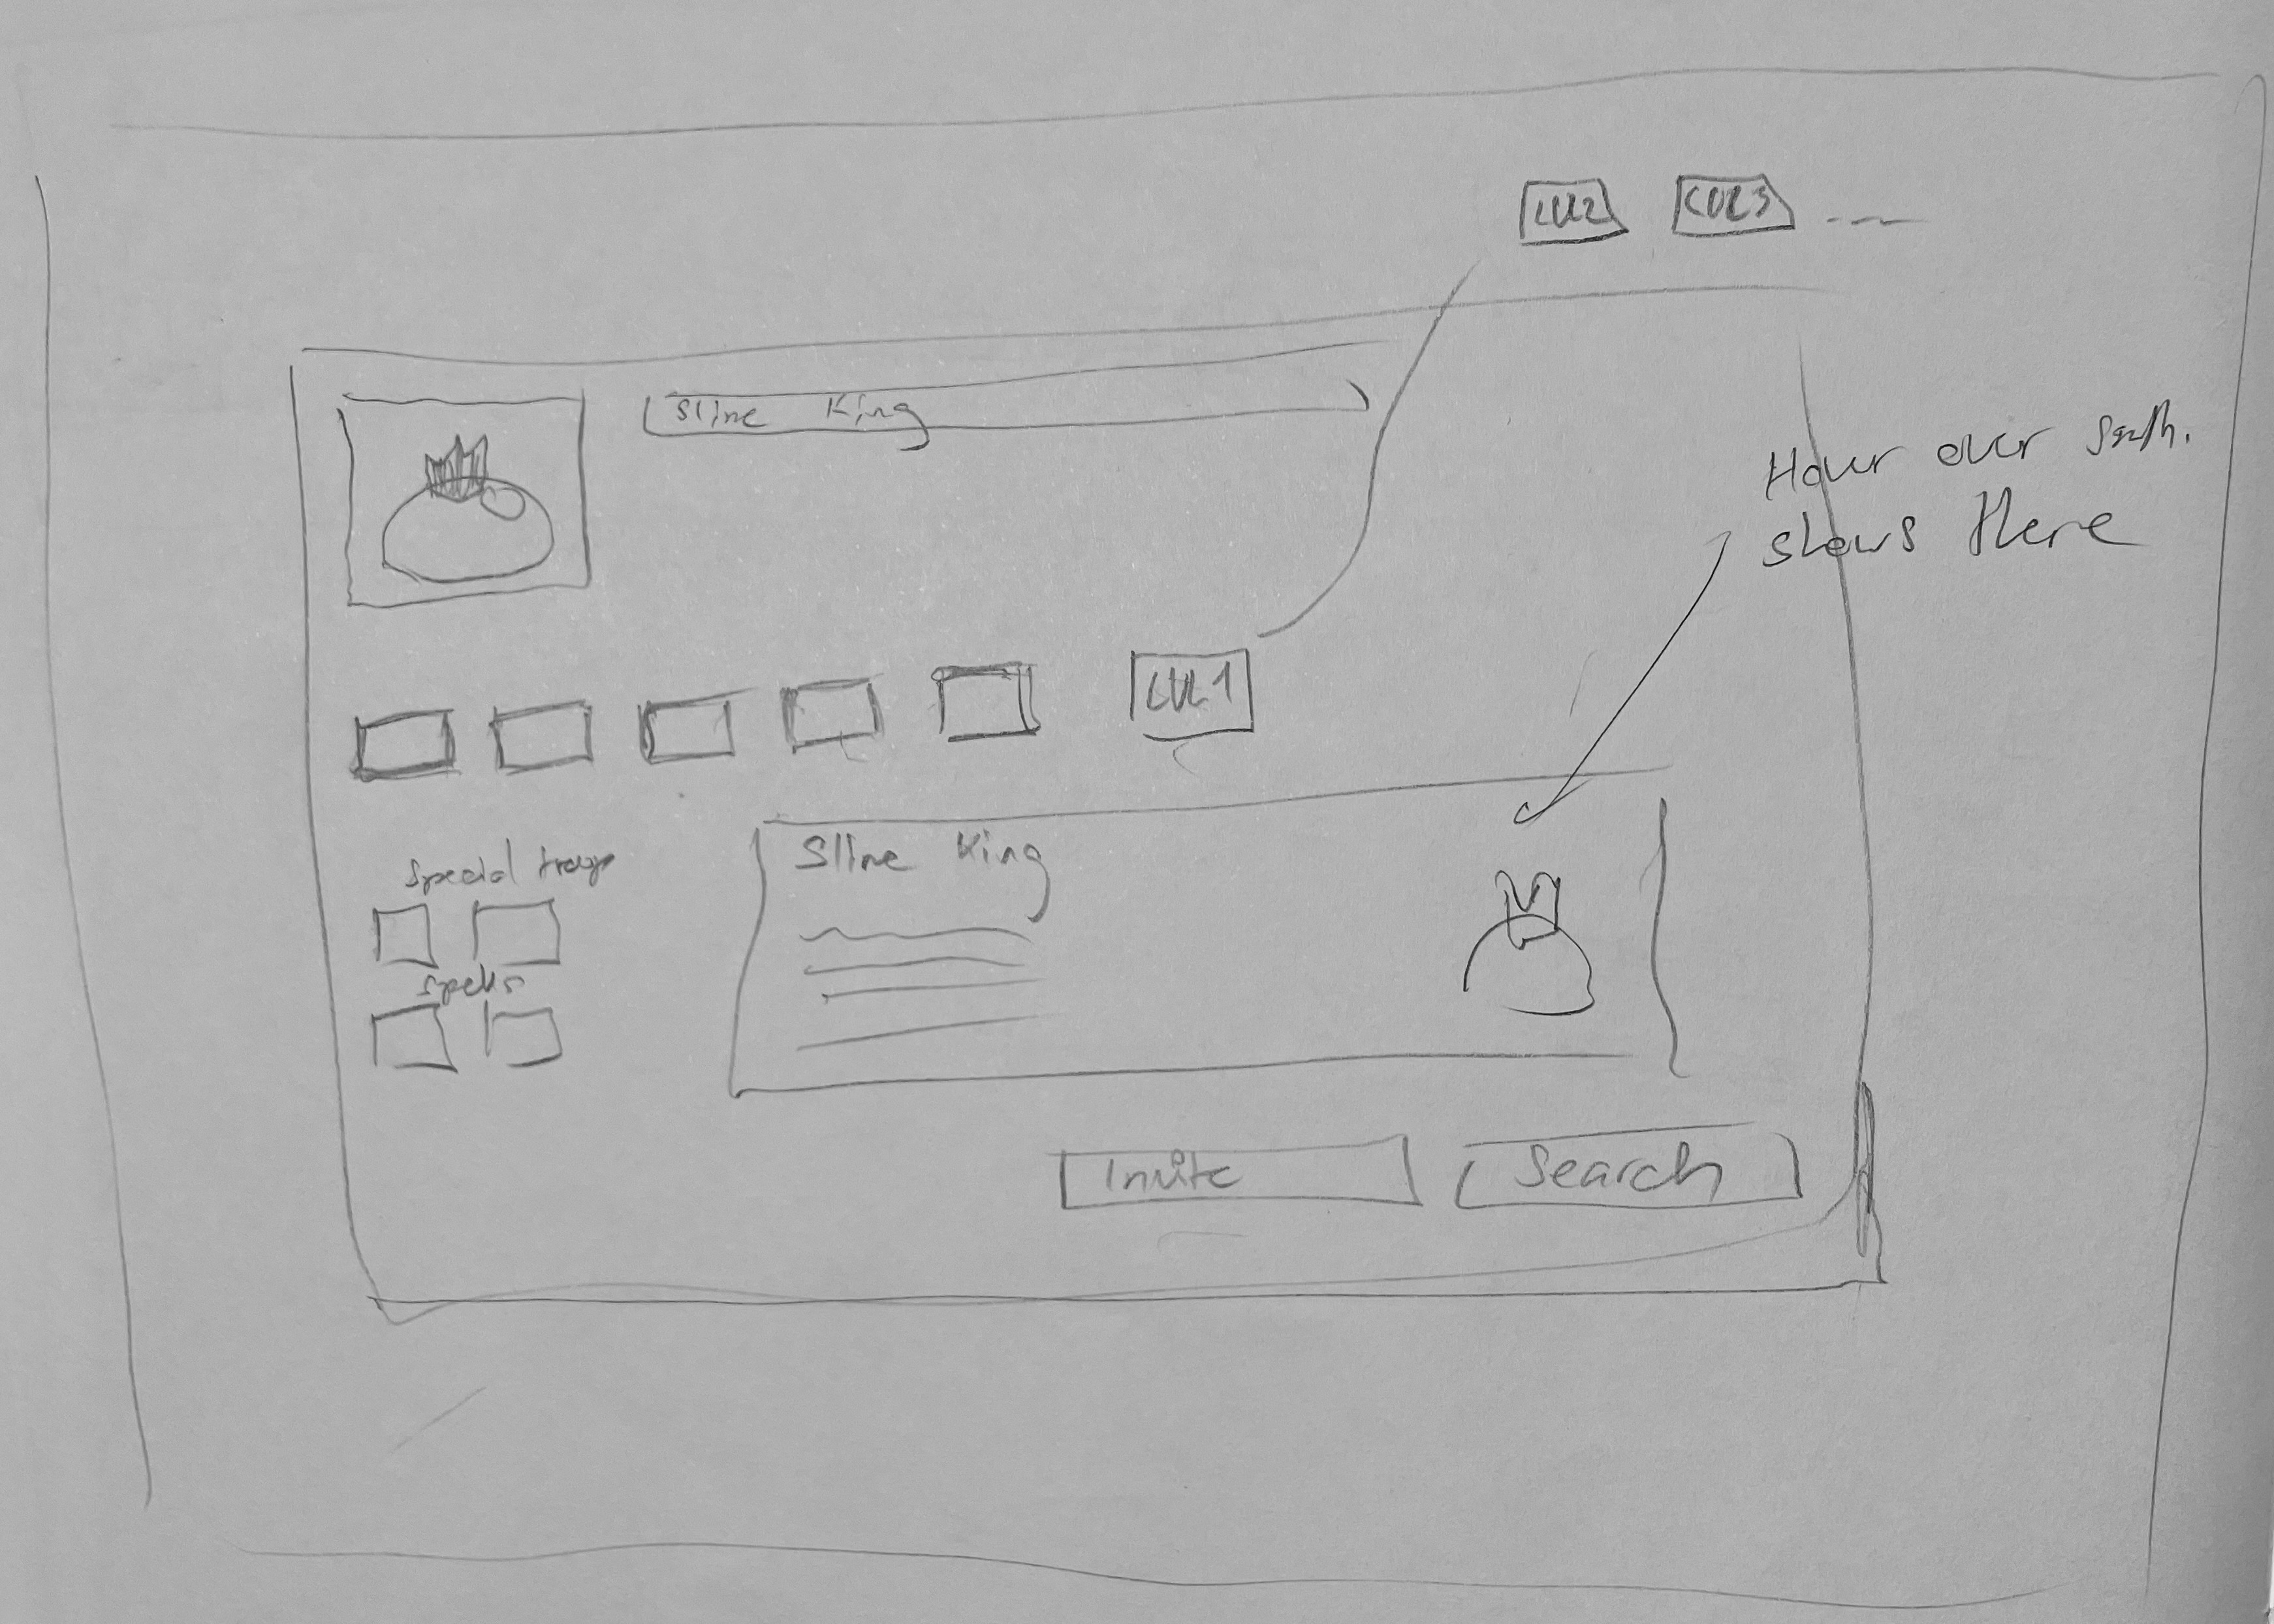
\includegraphics[width=7cm]{resources/SK_auswahl.jpeg}
    %    \caption{hello world} \caption{hello world}
    %\end{figure}
    %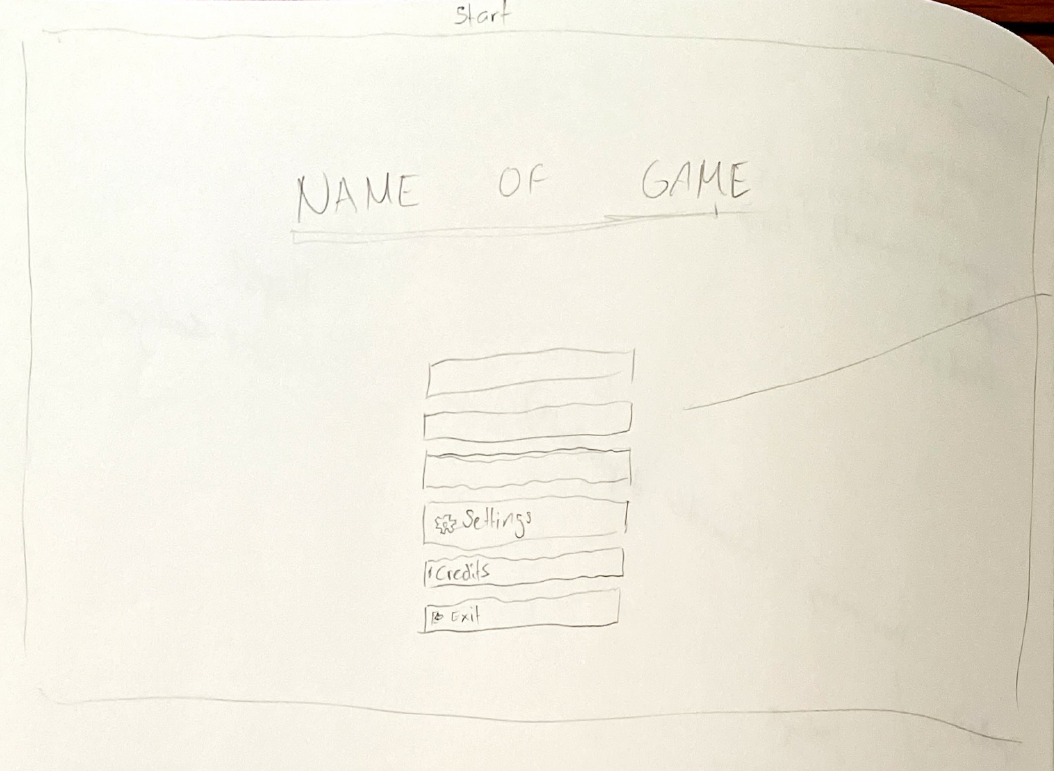
\includegraphics[width=7cm]{resources/SK_startpage.jpeg} \quad 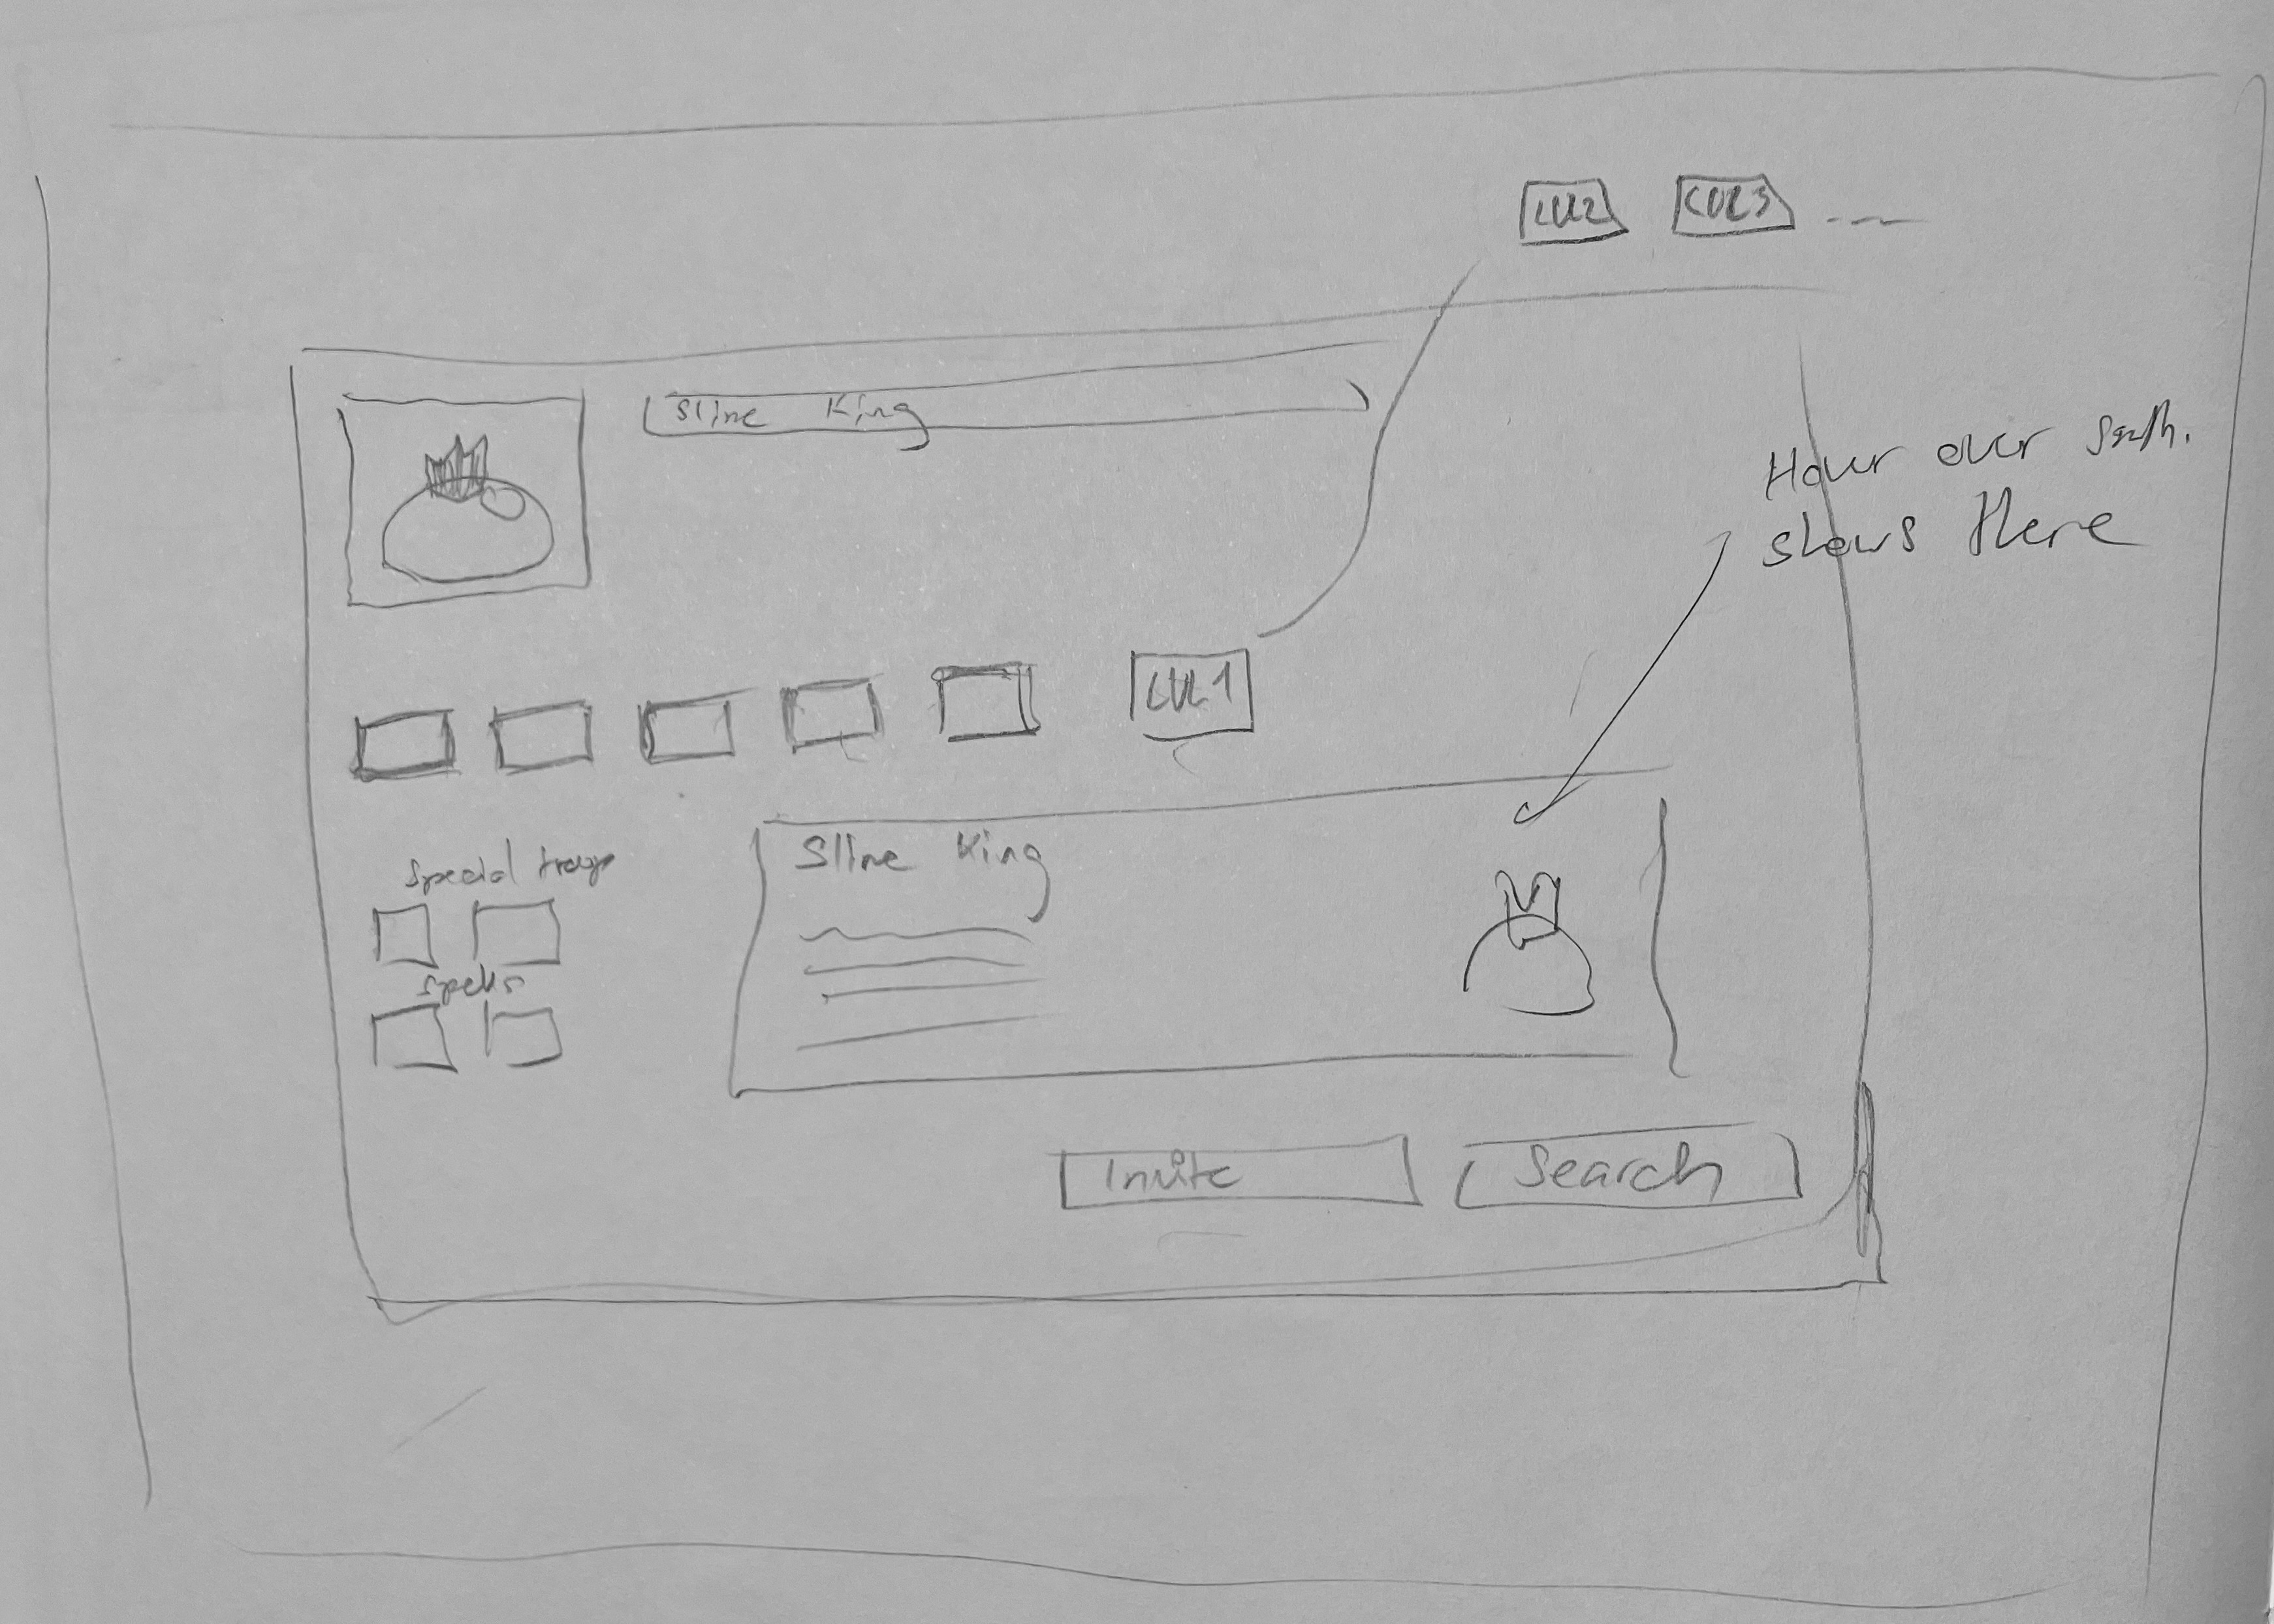
\includegraphics[width=7cm]{resources/SK_auswahl.jpeg}\\
    %\textit{Startseite} \qquad \qquad \qquad \qquad \qquad \qquad \qquad \quad \textit{Auswählen von Karten und Helden}
    \begin{figure}[H]
        \centering
        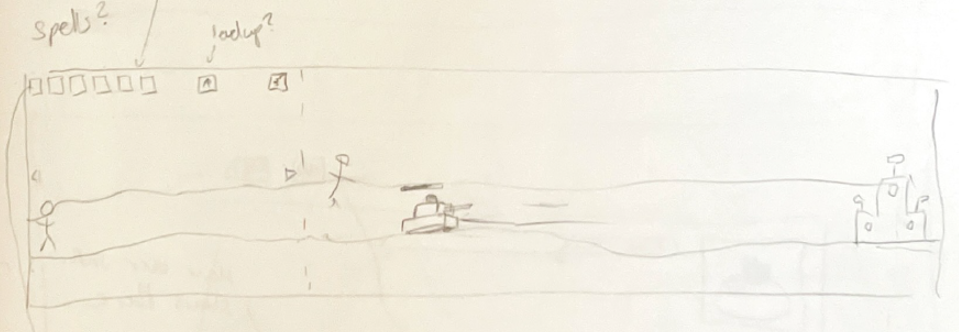
\includegraphics[width=14.5cm]{resources/sk_gamemain.jpeg}\\
        \caption{Spieleszene mit UI}
    \end{figure}

    \begin{figure}[H]
        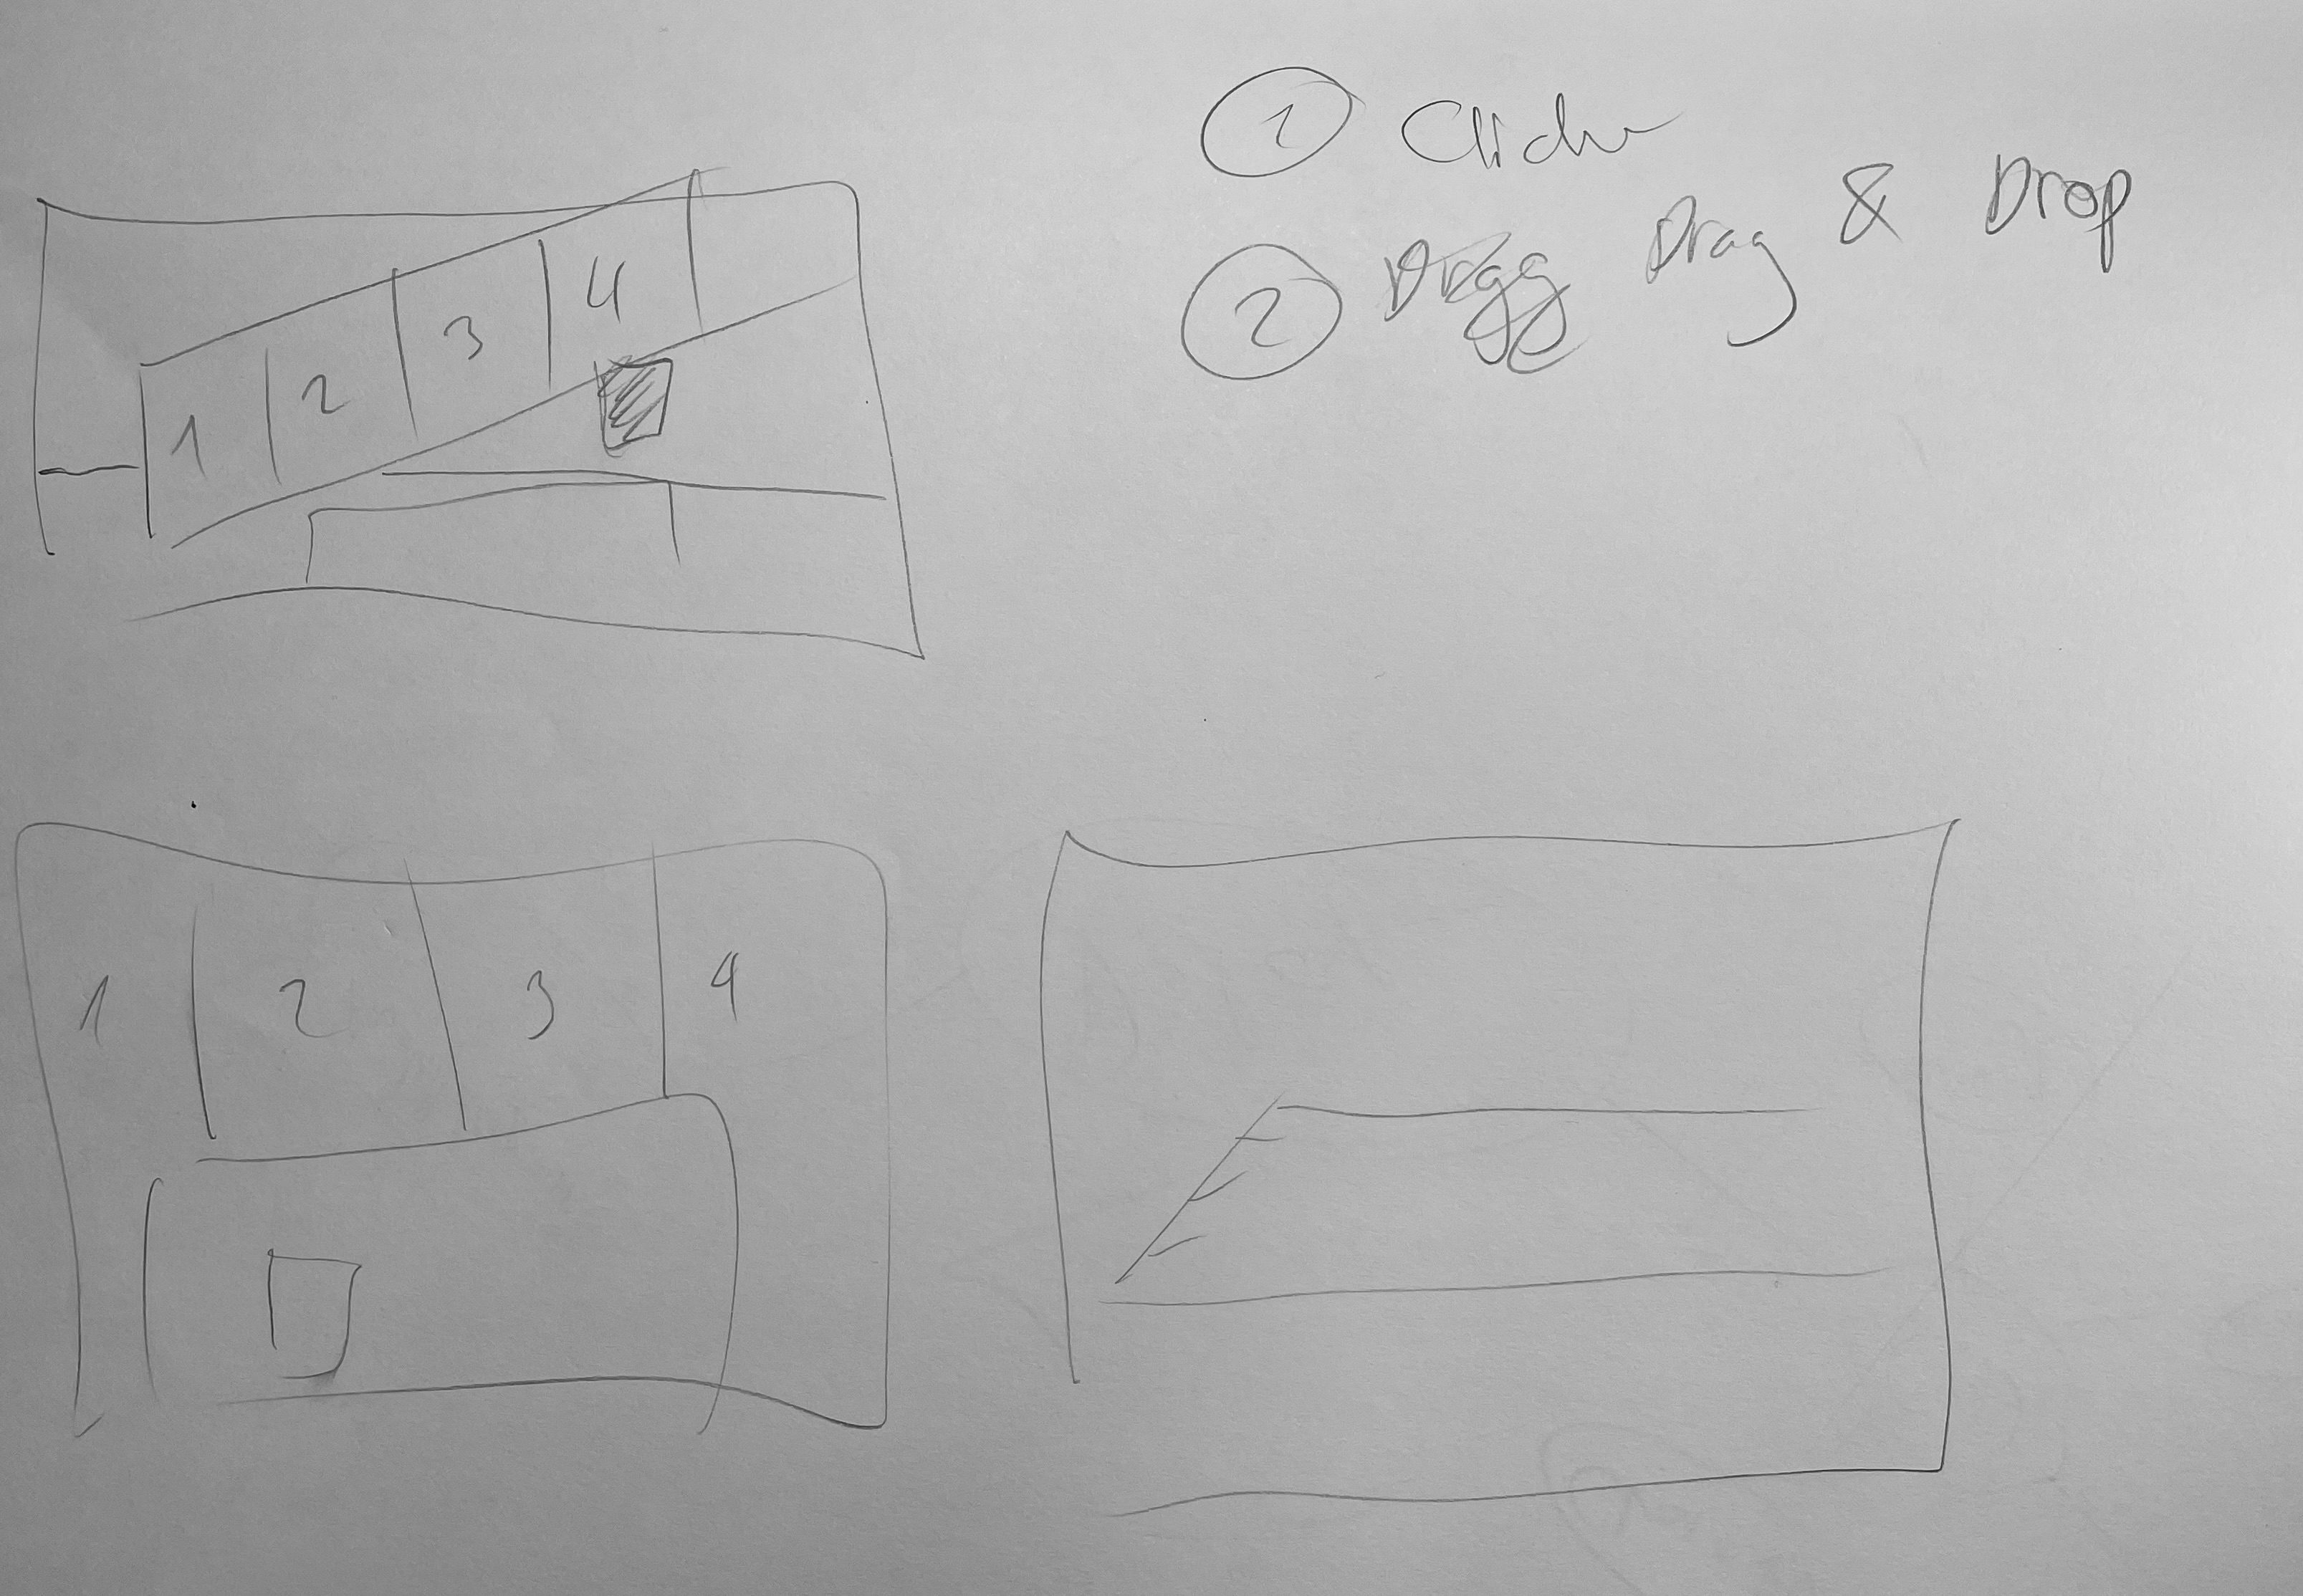
\includegraphics[width=14.5cm]{resources/Sk_dragndrop.jpeg}\\
        \caption{Mechanik der Karten / Spawnen von Truppen}
    \end{figure}

\section{Mindmap}
    \begin{figure}[H]
        \centering
        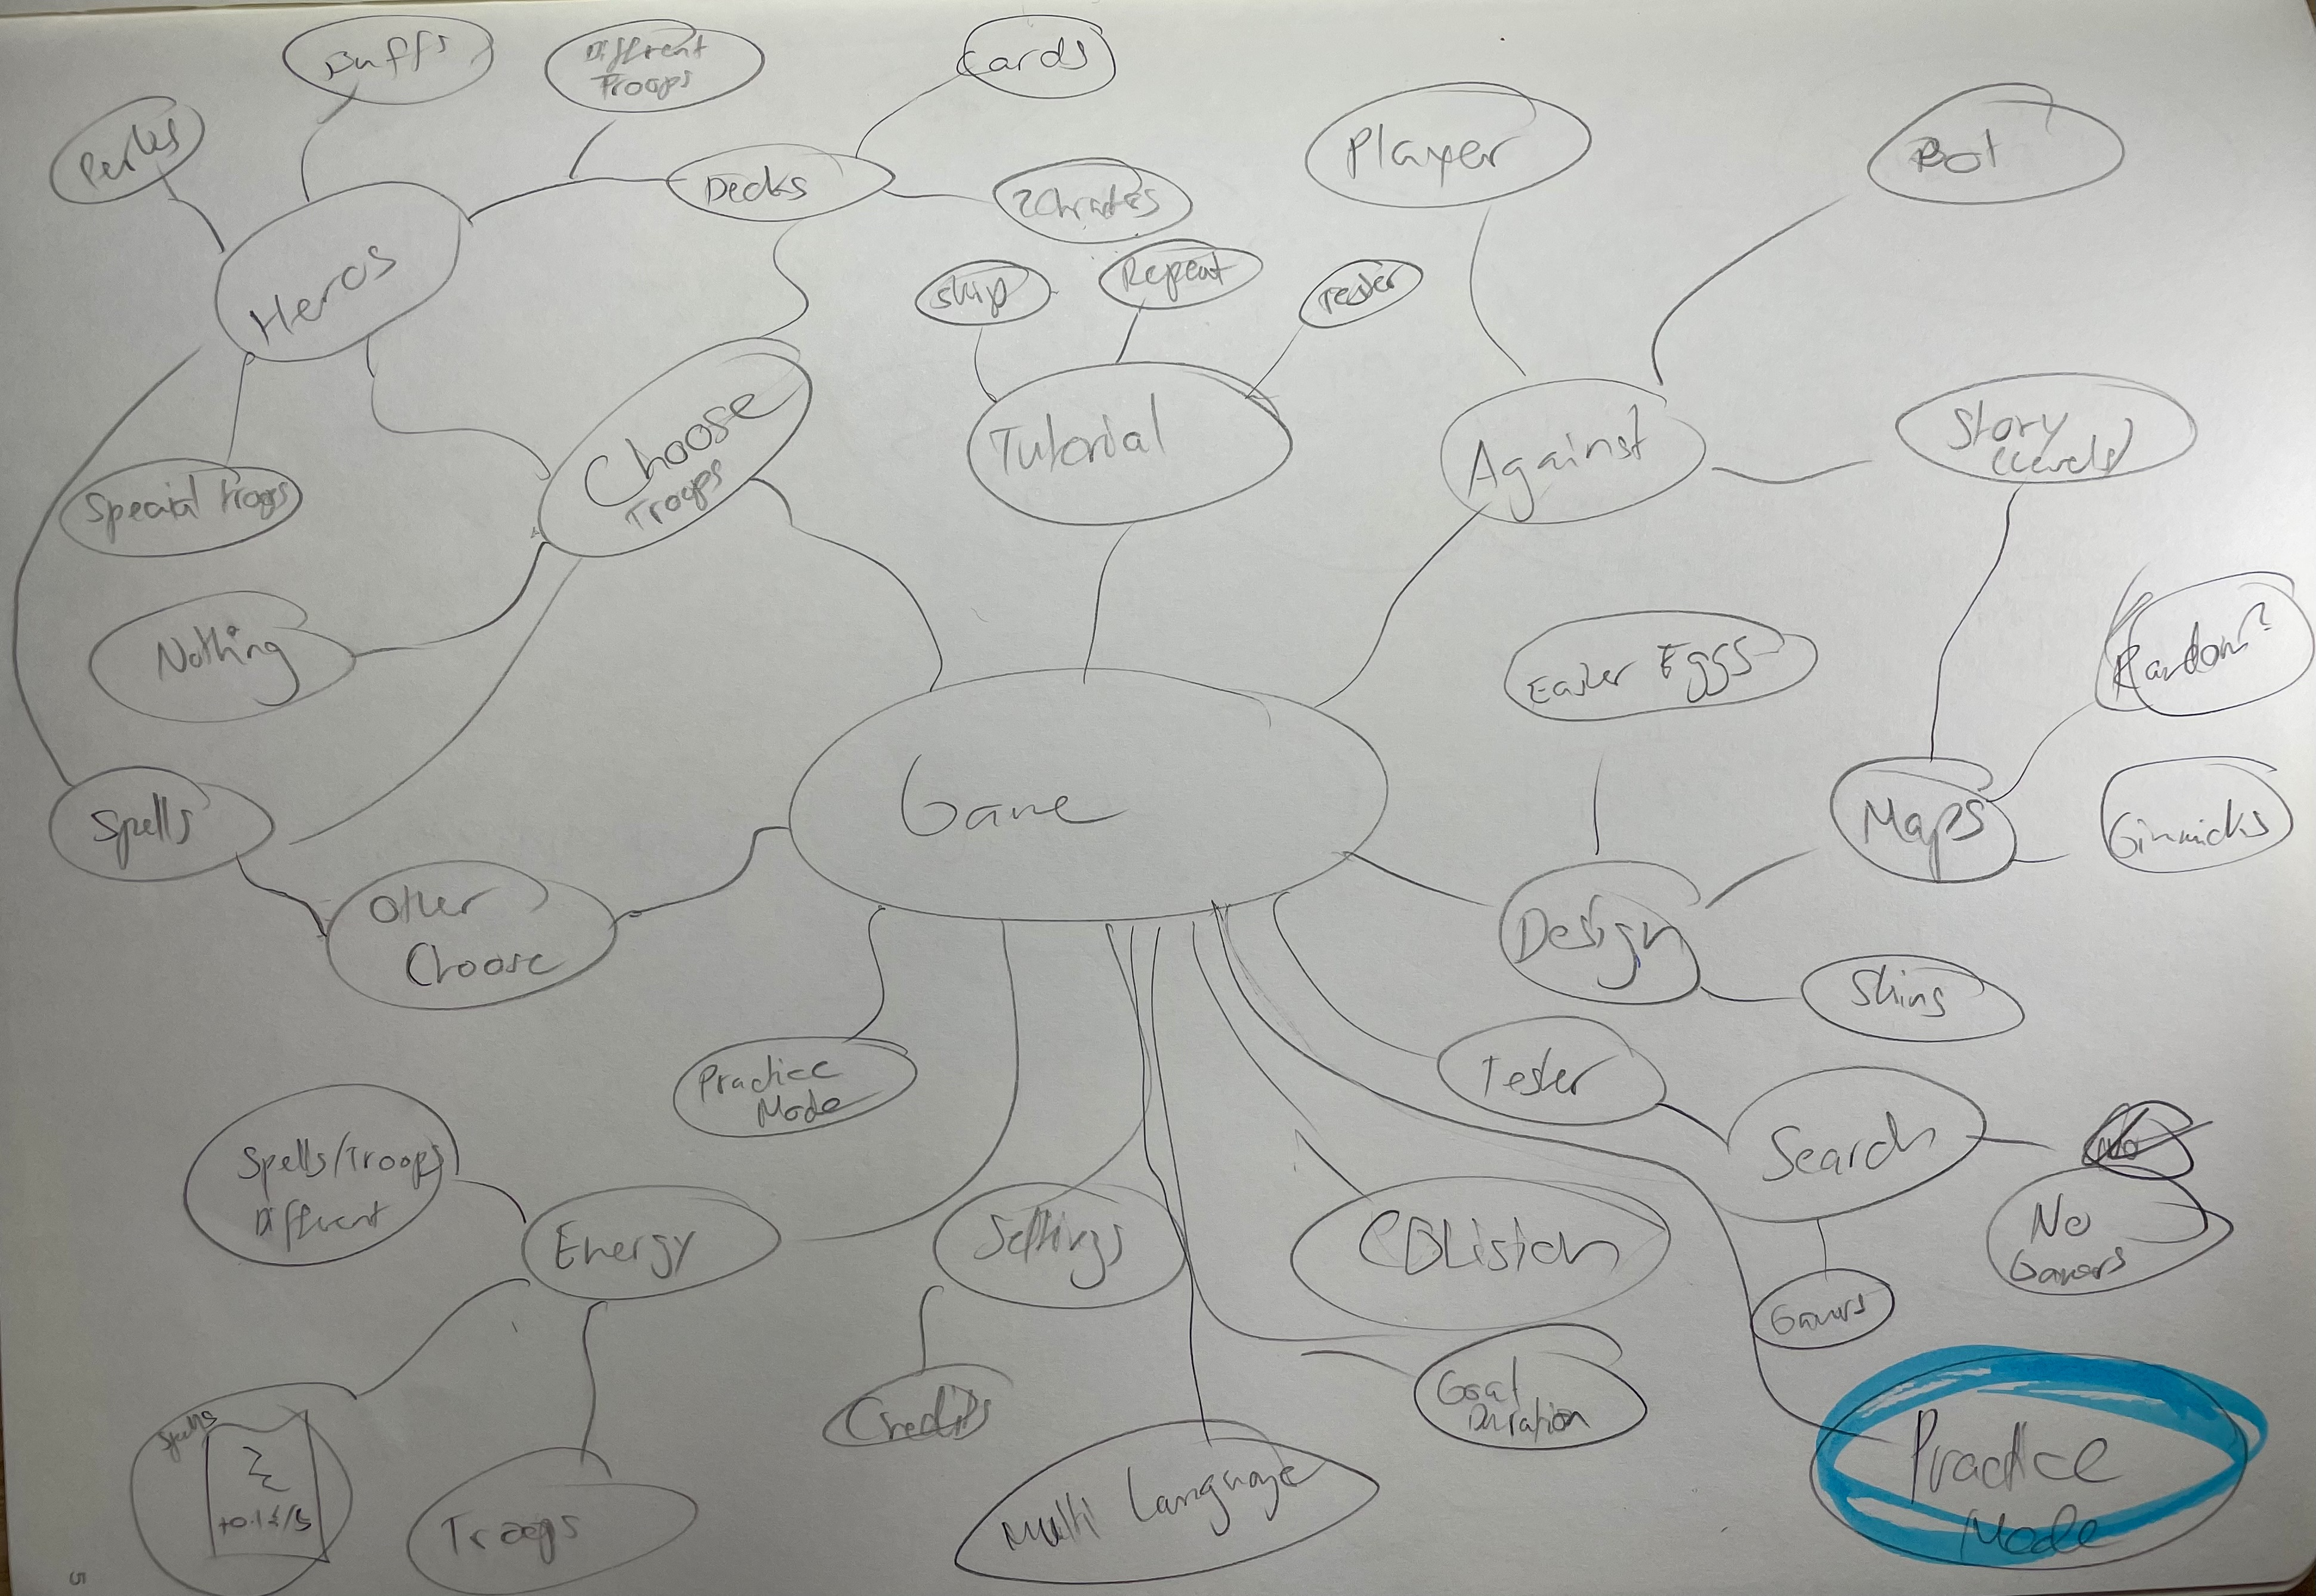
\includegraphics[width=14.5cm]{resources/Sk_mindmap1.jpeg}\\
        \caption{Mindmap}
    \end{figure}


\section{Überlegungen zum Spielprinzip}

Die Idee des Spielprinzips wird im folgenden Unterkapitel grob beschrieben.\
\begin{itemize}
    \item In unserem Spiel treten zwei Spieler*innen gegeneinander an. Dabei befinden sich die Startbereiche der Spieler*innen auf der linken bzw. rechten Seite einer steinernen Brücke.
    \item In die Schlacht begleitet wird jede*r Spieler von vier Helden. Diese Helden schreiten zu Beginn des Spieles durch die magischen Portale und bilden einen ersten Verteidigungswall.
    Sterben jene Helden, lösen sie einen Zauber aus, der alle gegnerischen Truppen auf dieser Linie der Brücke ausradiert.
    \item Der*die Spieler*in kann zudem Unterstützung aus dem eigenen Lager befehligen. Die verfügbaren Truppen erhält der*die Spieler*in in Form von Karten. Der*die Spieler*in kann mit der Verschiebung dieser Karten auswählen, durch welches Portal sie schreiten sollen.
    \item Jede Truppe verlangt eine unterschiedliche Menge an Kraft (Mana, spirituelle Energie), um das Portal zu durchschreiten. Die zur Verfügung stehende Mana wird oben recht angezeigt.
    \item Nach jeder Durchschreitung muss der*die Spieler*in eine bestimmte Zeit warten, bis er die nächste Truppe auswählen kann.
    \item Gelingt es einer verbündeten Einheit das gegnerische Portal zu durchschreiten, ist das Spiel vorbei und man hat gewonnen. 
    \item Mit den Pfeiltasten kann der*die Spieler*in steuern, welchen Teil des Schlachtfelds er überblicken will.
\end{itemize}



% \includegraphics[width=\textwidth]{resources/diagrams/domain-model}
